\section{Conformal Invariance}
\label{ch:conf}

In Section~\ref{sec:scaling} we talked about the principle of scale invariance
and how incredibly useful it is. It is based on the fact that the correlation
functions transform covariantly under a change in scale $\mathbf{r}\rightarrow
b\mathbf{r}$. A \textit{global} change in scale, that is. One could perfectly
construct a transformation in which the scaling factor $b$ depends on the
position $b=b(\mathbf{r})$. This would be a \textit{local} change of scale.
This kind of transformation would deform the overall shape of the system, but
in the direct vicinity of a point it would look like a regular scale
transformation with possibly a rotation and translation. Luckily there is a
class of functions that look exactly like that, these are called
\textit{conformal transformations}.

For the geometrists in the crowd, conformal transformations are coordinate
changes that keep the metric invariant up to a local scaling factor
\begin{equation}
    g_{\mu\nu}'\left(\mathbf{r}'\right)=
    \Omega\left(\mathbf{r}\right)g_{\mu\nu}\left(\mathbf{r}\right)
\end{equation}


As Domb~\cite{Domb1972} puts it
\begin{equation*}
    \left.\begin{array}{l}
            \mbox{Scale Invariance}\\
            \begin{array}{cl}
                + & \mbox{Translation Invariance}\\
                + & \mbox{Rotational Invariance}\\
                + & \mbox{Short-range Interactions}
            \end{array}
        \end{array}
    \right\} \Rightarrow\mbox{Conformal Invariance}
\end{equation*}

In $d>2$ the group of conformal transformations is finite dimensional, and
it is composed of only translations, rotations, dilations and the special
transformation
\begin{equation}
    \mathbf{r}\rightarrow\mathbf{r}'=
    \frac{\mathbf{r}+\mathbf{a}r^{2}}{1+2\mathbf{a}\cdot\mathbf{r}+a^{2}r^{2}}.
\end{equation}
These four transformations can be condensed into one in the complex plane
\begin{equation}
    w\left(z\right)=\frac{az+b}{cz+d},\;\;\;\;\;\;\;\; ad-bc=1.
\end{equation}
Unfortunately the projective transformations are not enough to determine the 

The stress-energy tensor transforms as
\begin{equation}
    \left\langle T\left(z_{1}\right)T\left(z_{2}\right)\right\rangle=
    \frac{c/2}{{\left(z_{1}-z_{2}\right)}^{4}},
\end{equation}
which define the \textit{central charge} $c$.


\begin{figure}
\begin{center}
    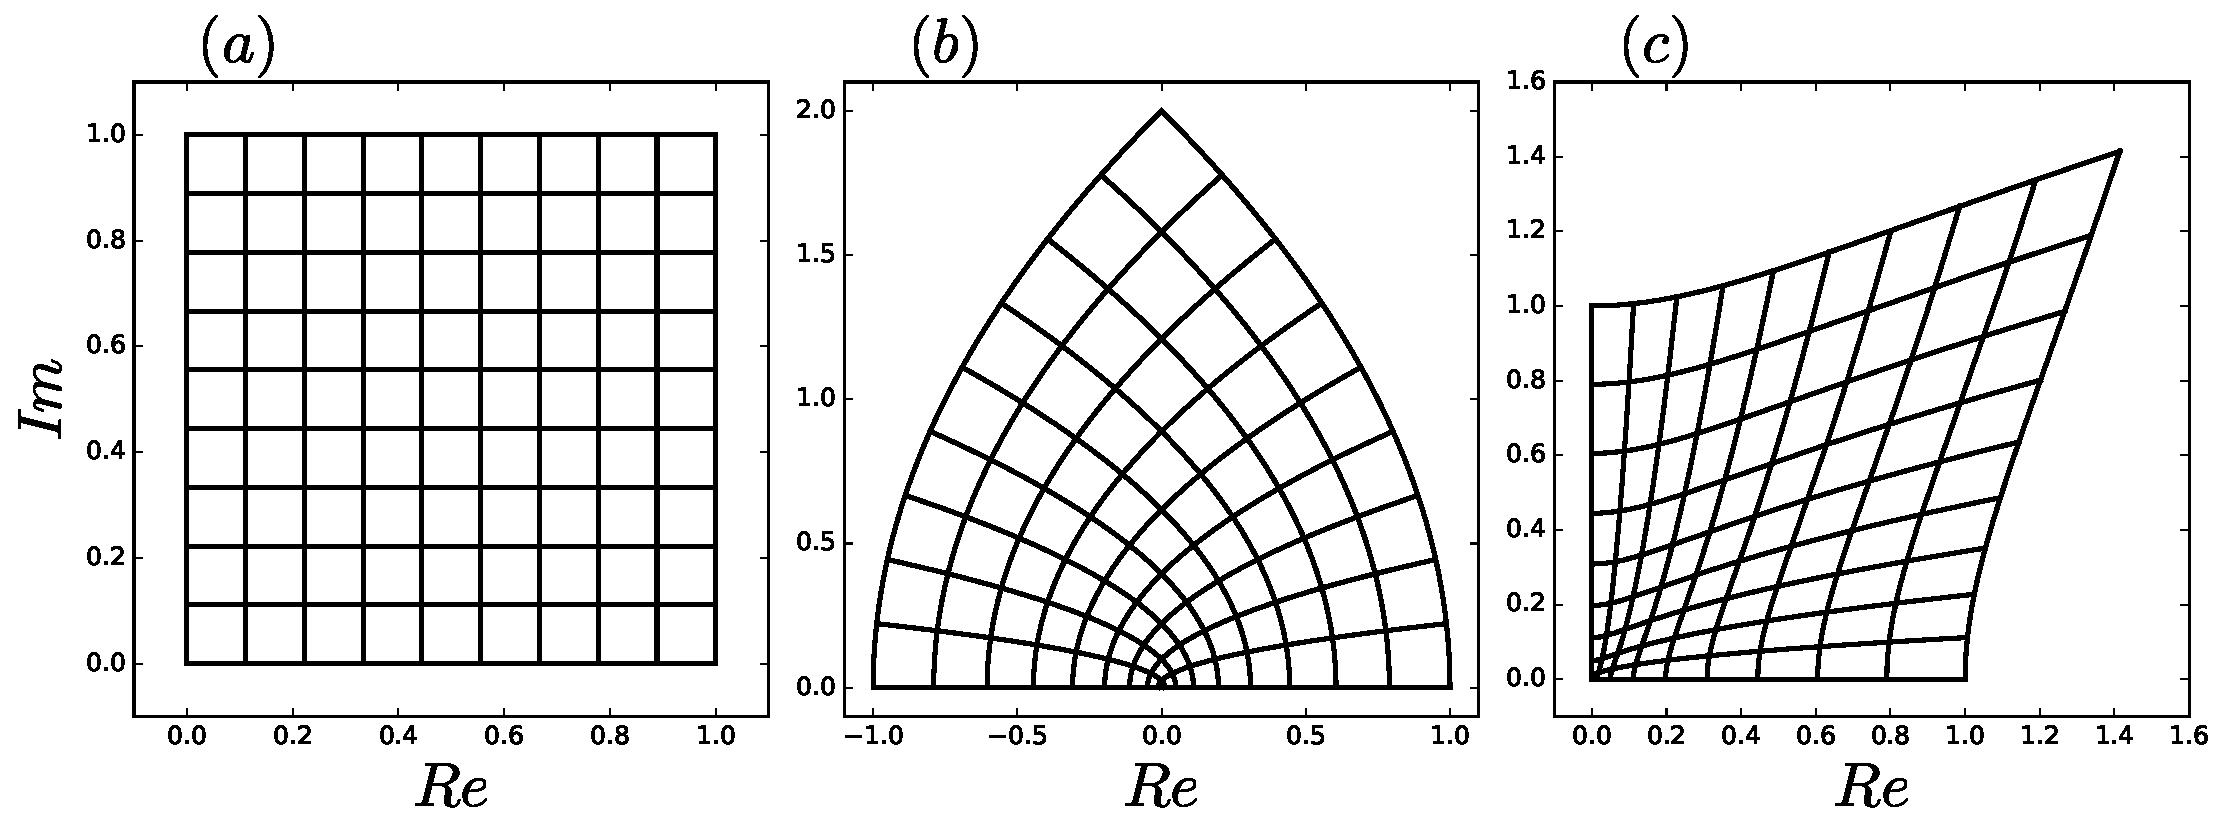
\includegraphics[width=\textwidth]{chapters/ch3-conf/figs/cmapex}
\end{center}
\caption{Coordinates transformations in the complex plane can be divided into
    conformal and non-conformal. Conformal transformations preserve the
    intersection angles between lines, unlike the non-conformal. The
    transformation from the square lattice in (a) into (b) is conformal
    ($f(z)=z^2$), while the one from (a) to (c) ($f(z)=z|z|$) is not.}
\label{fig:cmapex}
\end{figure}


\begin{figure}
\begin{center}
    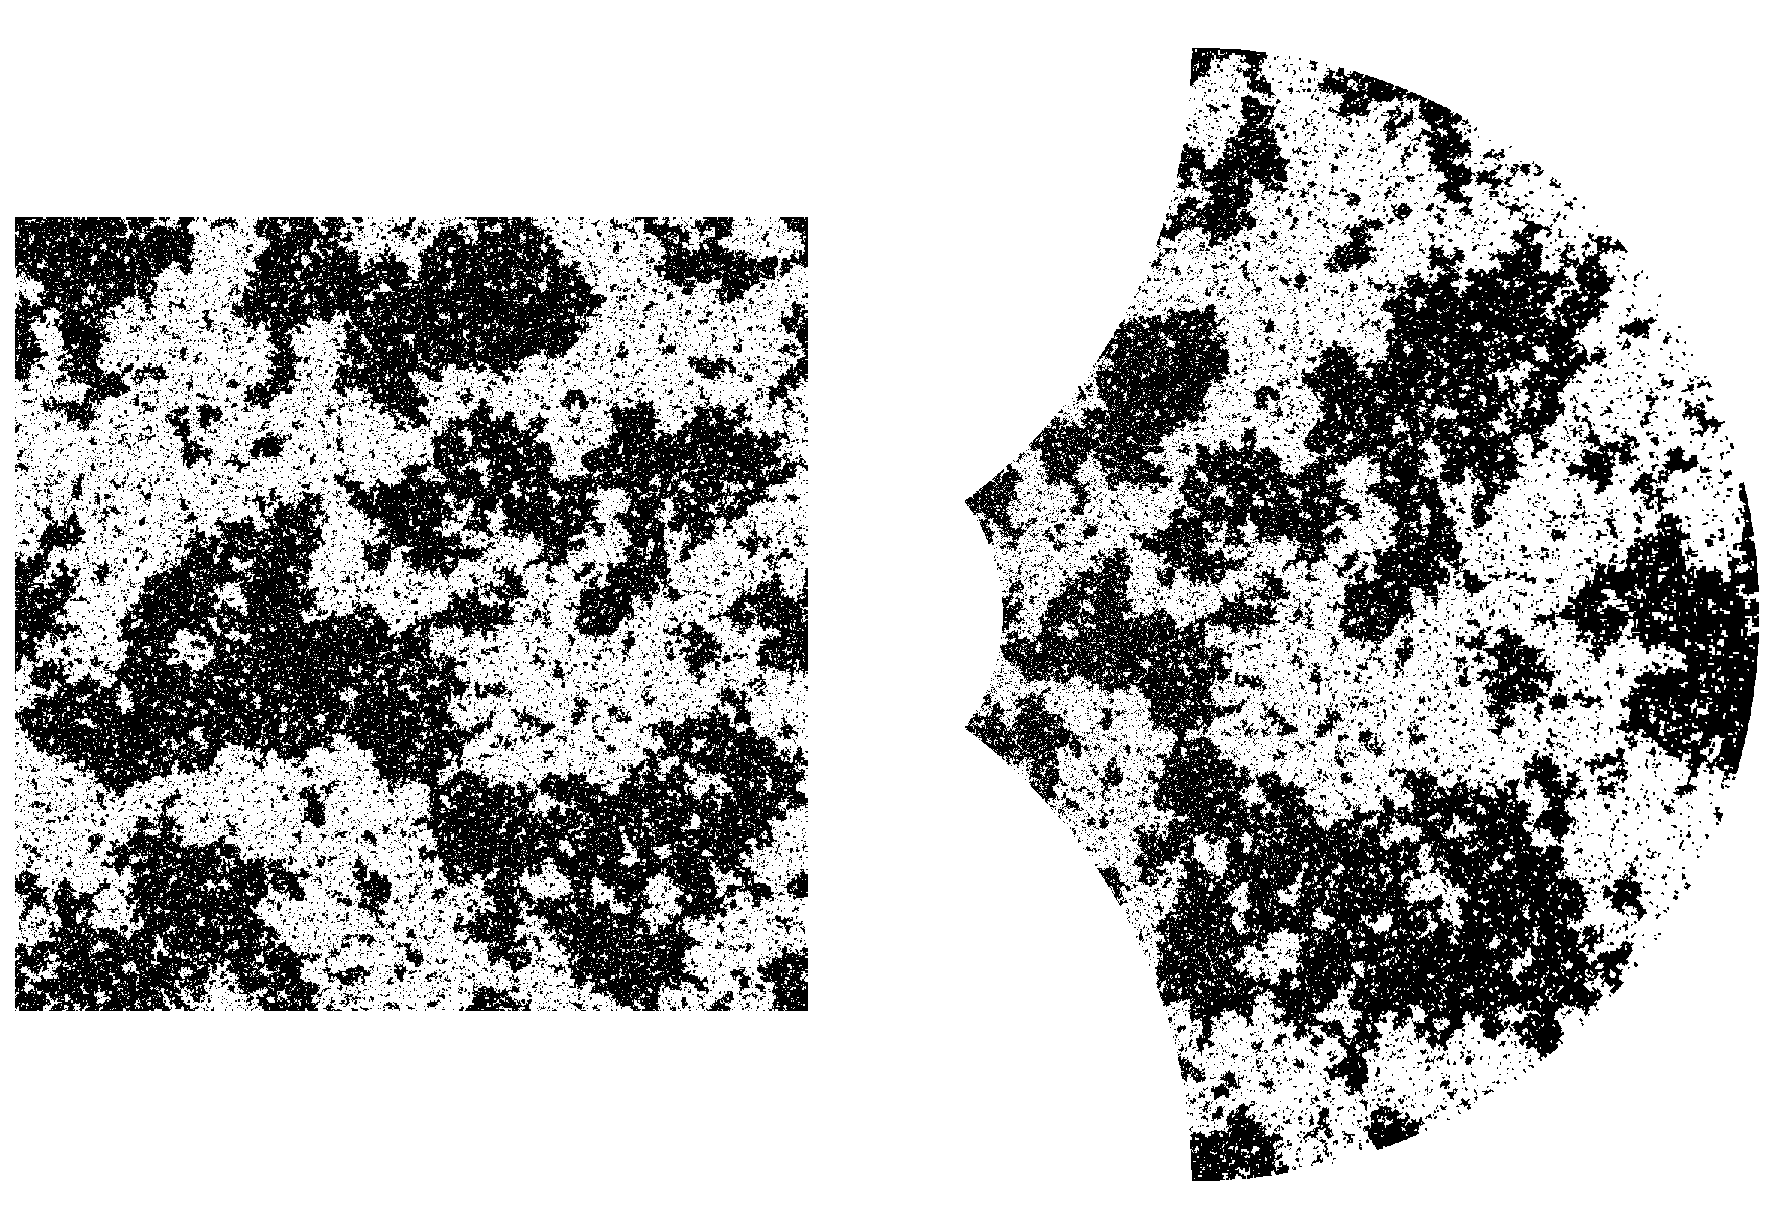
\includegraphics[width=0.8\textwidth]{chapters/ch3-conf/figs/isingcm}
\end{center}
\caption{Illustration of the Ising model at the critical point when transformed
    under a conformal map $f(z)=z/(2-z)$. The deformed image still looks
    statistically similar to the original, which is a consequence of conformal
    invariance.}
\label{fig:isingcm}
\end{figure}

\begin{figure}
\begin{center}
    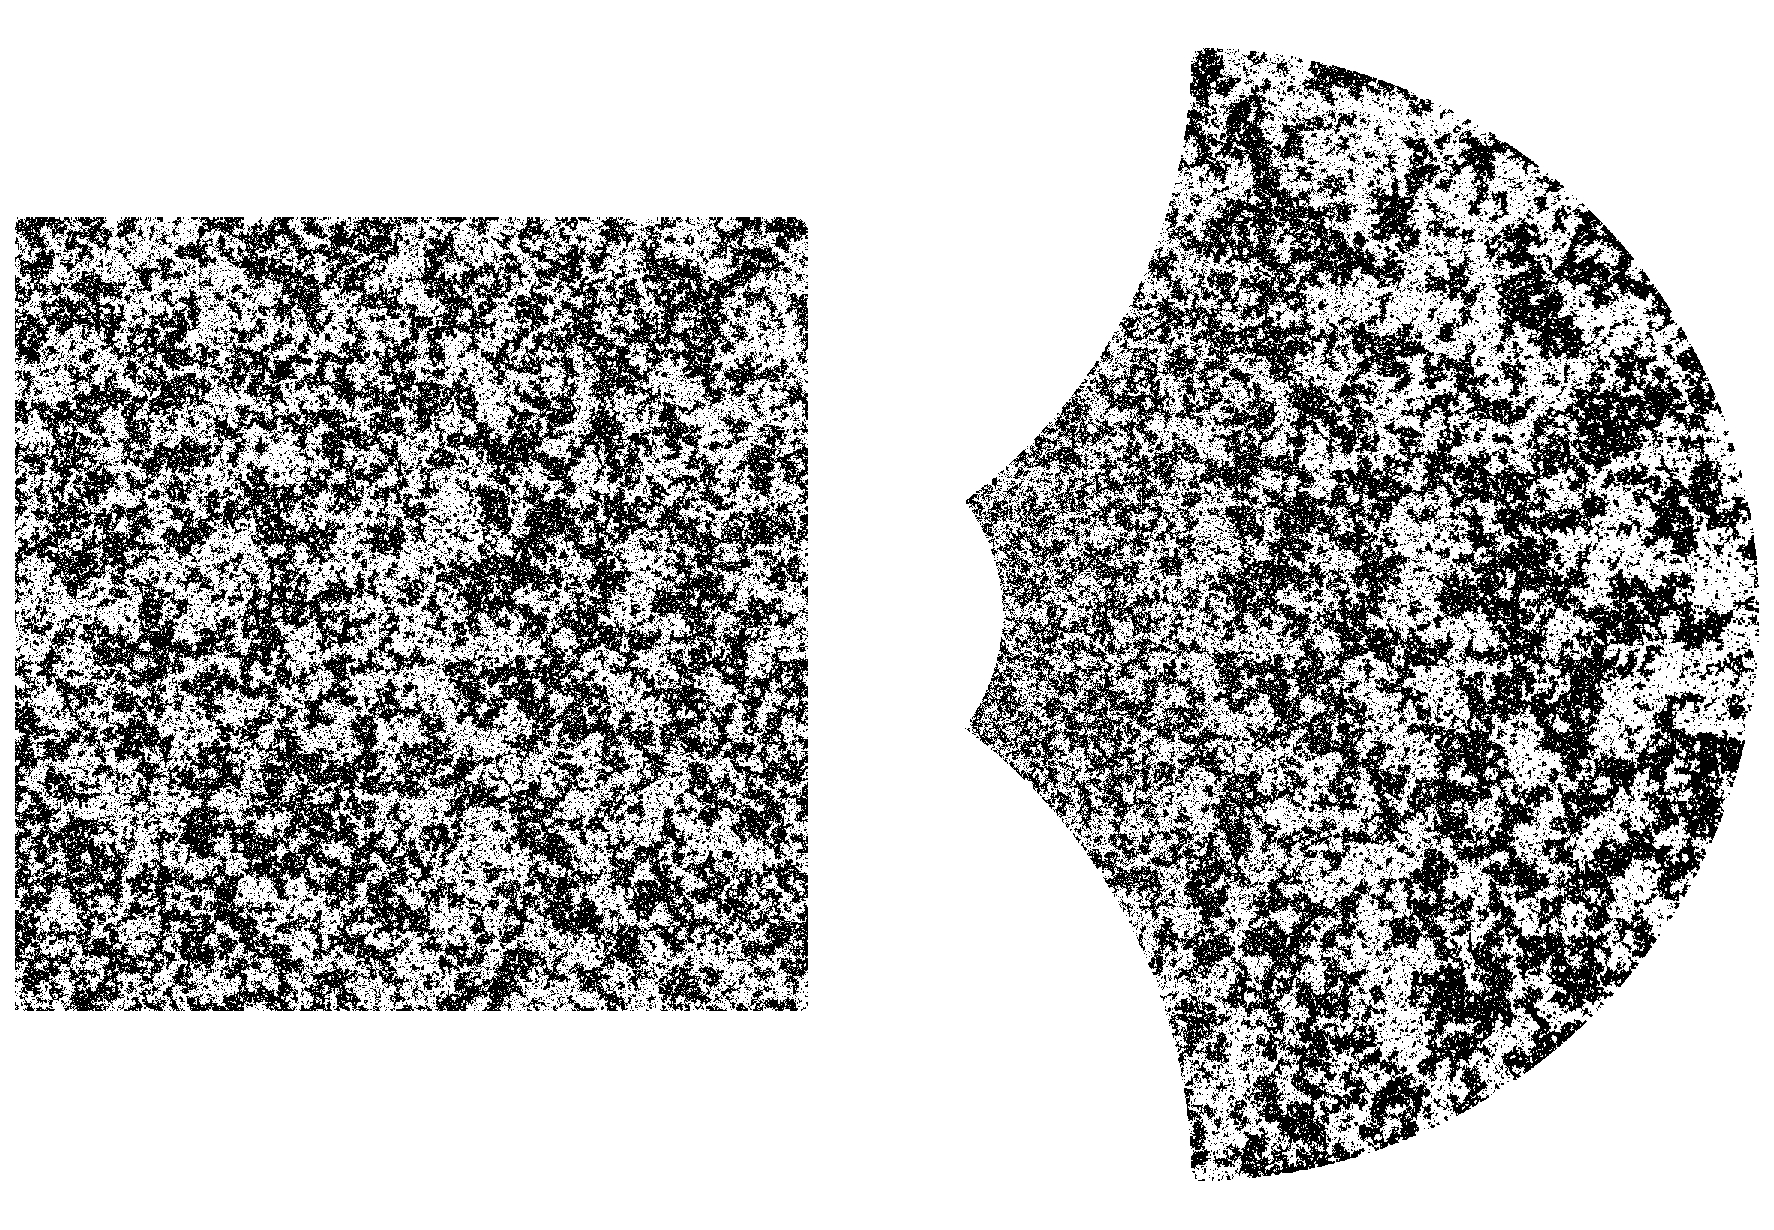
\includegraphics[width=0.8\textwidth]{chapters/ch3-conf/figs/isingcm2}
\end{center}
\caption{Illustration of the Ising model above the critical point when
    transformed under a conformal map $f(z)=z/(2-z)$. In the deformed image,
    the spin configuration is no longer homogeneous, because outside the
    critical point the system is no longer conformally invariant.}
\label{fig:isingcm2}
\end{figure}
